\documentclass[12pt]{article}
\usepackage[margin=2cm]{geometry}

% for links
\usepackage{hyperref}

% to include images
\usepackage{graphicx}

% for equation environments
\usepackage{amsmath}

% For header and footer
\usepackage{fancyhdr}
\usepackage{float} % formats figures
\pagestyle{fancy}
\fancyhf{} % clears default style
\lhead{F21BC Biologically Inspired Computation}
\lfoot{Kyle Mckay (km2008), Lina Rietuma (lr2004)}
\cfoot{\thepage}
\rfoot{HWU Person IDs: H00358352, H00361943}
\renewcommand{\headrulewidth}{0pt}

% No paragraph indentation
\setlength\parindent{0pt}
\setlength\parskip{1em}
\raggedright

\begin{document}

\title{Particle Swarm Optimisation for Artificial Neural Network Training}

\begin{center}
  \Large{Particle Swarm Optimisation for Artificial Neural Network Training}
\end{center}

\vspace{-2em}
\section{Introduction}
\vspace{-1.5em}

The following specifies the implementation of a particle swarm
optimisation (PSO) algorithm and its subsequent use in training an
artificial neural network (ANN) to fit a binary classification dataset.
PSO hyperparameters are investigated in an effort to improve search
space exploration and thus classification performance. Finally, PSO is
compared to back-propagation as an alternative approach for ANN training
and solving the given classification problem.

\vspace{-1.5em}
\section{Program development rationale}
\vspace{-1.5em}

Following on from the ANN implementation, PSO was also implemented in
Python using NumPy for efficient updates to particle positions and velocities.
The implementation consists of a \texttt{particle} class which contains
the logic to update positions and velocities at each search iteration.
A PSO swarm can be instantiated as the \texttt{swarm} class, which provides
methods to set PSO hyperparameters and initiate a search.

For quality of life, the fitness metric used in PSO is not hard-coded
into the \texttt{swarm} class. This means the PSO code is not coupled to
a specific search problem and is more generally usable. By default, the
sphere function is used for fitness since it works in \(n\) dimensions
and is a simple test case.

The swarm particles are initialised uniformly throughout the search space
by distributing a shared uniform vector of values. Their initial velocities
are set in accordance with SPSO 2011 \cite{Clerc} to discourage them from
immediately leaving the search space. A ring topology \cite{Clerc} is used to
ensure there is an adequate linkage for information to propagate through
the swarm.

During search, the ``absorbing'' \cite{Chu} boundary enforcement scheme is used
for simplicity. Other schemes were tried (e.g. random, reflecting) and
found to have little effect.

A static \texttt{from\_list} method is added to the \texttt{network}
class that converts an appropriate length \texttt{numpy.ndarray}
into a set of weights and activation functions for a \texttt{network} instance. In this way, a particle's current position
can represent an ANN that can be used with the dataset to produce a
fitness value (loss, accuracy, etc.).


\vspace{-1.5em}
\section{Methods}
\vspace{-1.5em}

To ensure a fair comparison between back-propagation and PSO models, the same baseline architecture of 2 layers with 4 nodes each is used. To find the optimal PSO configuration the following hyper-parameters were formally investigated: swarm size, search space limits, inertia weight, acceleration coefficients, and step size. Additionally, different deltas, numbers of iterations, fitness metrics, ANN architectures and search problems were explored in an attempt to improve PSO's performance.

Swarm sizes are tested in the range from 10 to 100 particles. The optimal swarm size is problem-dependent, heavily influenced by the dimensionality of the problem \cite{Razee}. From SPSO 2006, \(S = 10 + 2\sqrt{D}\) is used for determining the optimal swarm size (implies a swarm of 24 particles for the dimensionality of this problem) while SPSO 2011 suggests using 40 particles \cite{Clerc} -- the default used here. Given the perceived complexity of the problem search space, the larger swarm sizes were introduced.

Inertia weight determines the proportion of the original velocity to be retained. Suggested values range from a minimum of \(0.2\sim0.4\) to a maximum of \(0.9\sim1.2\) \cite{Razee} \cite{Gudise}, hence the decision to test values around this range.

Literature search suggests that a relatively large beta (cognitive component) with respect to gamma (social component) can result in excessive wandering within the problem space -- while the reverse can lead to prematurely settling on a local minimum \cite{Kennedy}. These findings motivate the choice for approximately equal values of beta and gamma to yield the most effective search of the problem space.

Gudise et al (2003) suggest that an overly restricted search space (e.g. in the range -1 to 1) prevents particles from finding the global minima. They find rapid improvements in the time to convergence as the search range is increased, with optimal range (-100, 100) \cite{Gudise}. From experiments with back-propagation, optimal weight values are found to be within (-1, 1), therefore the suggested range of (-100, 100) was tested as the upper range.

\vspace{-1.5em}
\section{Results}
\vspace{-1.5em}


\begin{figure}[H]
  \centering
  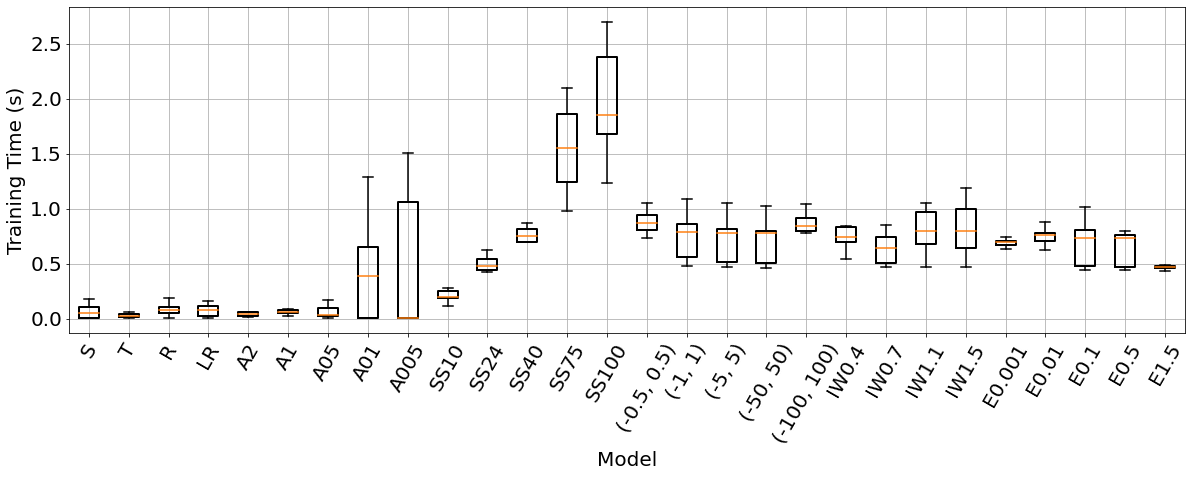
\includegraphics[width=1\textwidth]{figs/combo_ttime.png}
  \vspace{-1.5em}
  \caption{
    Average training time of each model across 10 iterations.
    Modified hyper-parameter abbreviation identifies each model:
    S|T|R|LR = activation function, A = learning rate for back-propagation models,
    SS = swarm size, () = search range, IW = inertia weight, E = step size.
  }
  \label{fig:ttime}
\end{figure}

\begin{figure}[H]
  \centering
  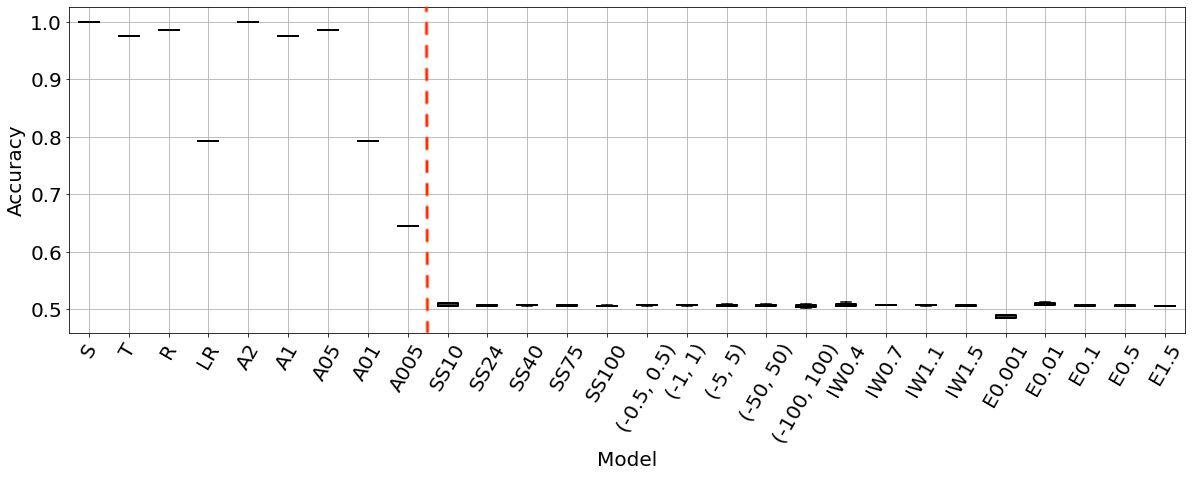
\includegraphics[width=1\textwidth]{figs/combo_acc.png}
  \vspace{-1.5em}
  \caption{
    Average accuracy of each model across 10 iterations.
    Modified hyper-parameter abbreviation identifies each model:
    S|T|R|LR = activation function, A = learning rate for back-propagation models,
    SS = swarm size, () = search range, IW = inertia weight, E = step size.
  }
  \label{fig:accuracy}
\end{figure}


\begin{figure}[H]
  \centering
  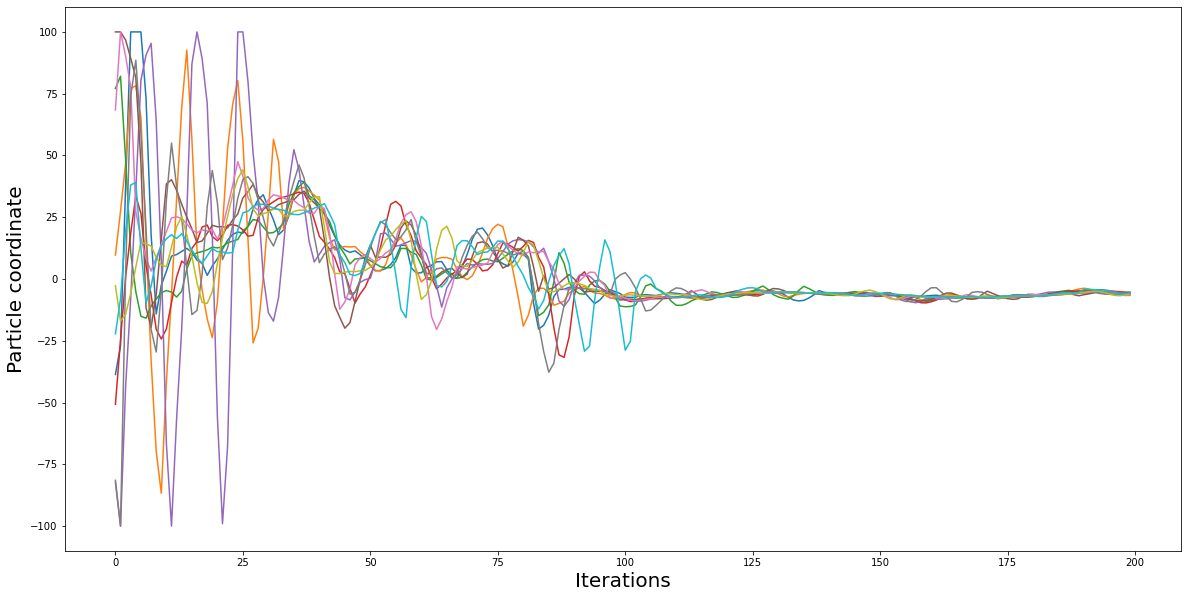
\includegraphics[width=0.9\textwidth]{figs/sphere_pso.png}
  \vspace{-1em}
  \caption{Positions (in the first dimension) of 10 particles in a PSO swarm applied to the 70 dimensional Sphere function.}
  \label{fig:sphere}
\end{figure}

\vspace{-1.5em}
\section{Discussion}
\vspace{-1.5em}

Expectedly, more complex PSO implementations increase ANN's training time with swarm size contributing heavily to longer training. Given that each particle represents a separate neural network, it was predicted that back-propagation models would outpace PSO as is reflected in the results (Figure \ref{fig:ttime}).

PSO-trained ANNs are evidently under-performing also in terms of classification accuracy, with top accuracy of only  $\sim$51\%  (Figure \ref{fig:accuracy}). Similarly low accuracies, regardless of PSO hyper-parameter combination used, suggest that PSO particles easily get stuck in a local optima. It is observed, as shown in Figure \ref{fig:sphere}, that PSO is able to find the global minima at the origin point of the simpler Sphere function test case.

To improve PSO's performance, alternative fitness metrics were tested. A switch from classification accuracy to cross-entropy loss value was made to capture a more detailed change in ANN's performance as the particles move through search space.  An observation that all input instances are classified as the dominant class (i.e. the class with more instances) motivated the switch to a fitness metric insensitive to class size  imbalances -- i.e. Matthew's Correlation Coefficient (MCC). Using MCC prevents classifying all inputs as a single class, however the overall accuracy was not improved.

Luke (2013) suggests particle step size is most commonly set to 1 \cite{Luke}. However, a range of epsilon values from 0.001 to 1.5 is tested because of the observed swarm behaviour and seeming affinity to local optimums. It is theorised that this could be explained by the particles overshooting the global optima in a complex search landscape. Unfortunately, the different step sizes had no success in terms of improving classification accuracy.

\vspace{-1.5em}
\section{Conclusions}
\vspace{-1.5em}

PSO's seeming lack of responsiveness to any hyper-parameter changes prevents any meaningful conclusions from being made about the optimal hyper-parameter combinations -- any effects are cancelled out by the swarm getting bound to a local optima. Despite research evidence of PSO being as efficient as backpropagation (if not better) and PSO trained ANNs generalising better to unseen data \cite{Kennedy}, our results do not support the same conclusion. Based on the classification accuracies and training times, back-propagation is by far a better approach for ANN training for the given classification problem.

\vspace{-1.5em}
\begin{thebibliography}{10}

\bibitem{Chu} W. Chu, X. Gao, S. Sorooshian, 2011, ``Handling boundary constraints for particle swarm optimization in high-dimensional search space'', doi: 10.1016/j.ins.2010.11.030
\bibitem{Luke} Sean Luke, 2013, ``Essentials of Metaheuristics", Lulu, second edition, available at http://cs.gmu.edu/∼sean/book/metaheuristics/
\bibitem{Kennedy} J. Kennedy, R. Eberhart, 1995, ``Particle swarm optimization," Proceedings of ICNN'95 - International Conference on Neural Networks,  pp. 1942-1948 vol.4, doi: 10.1109/ICNN.1995.488968.
\bibitem{Razee} A. Rezaee Jordehi, J. Jasni, 2013, ``Parameter selection in particle swarm optimisation: a survey, Journal of Experimental \& Theoretical Artificial Intelligence", 25:4, 527-542, DOI: 10.1080/0952813X.2013.782348
\bibitem{Clerc} Maurice Clerc, 2012, ``Standard Particle Swarm Optimisation", hal-00764996
\bibitem{Gudise}  V. G. Gudise, G. K. Venayagamoorthy, 2003, ``Comparison of particle swarm optimization and backpropagation as training algorithms for neural networks," Proceedings of the 2003 IEEE Swarm Intelligence Symposium. SIS'03 (Cat. No.03EX706), pp. 110-117, doi: 10.1109/SIS.2003.1202255.


\end{thebibliography}

\end{document}
